%%%%%%%%%%%%%%%%%%%%%%%%%%%%%%%%%%%%%%%%%%%%%%%%%%%%%%%%%%%%%%%%%%%
%                                                                 %
%                            CHAPTER FOUR                         %
%                                                                 %
%%%%%%%%%%%%%%%%%%%%%%%%%%%%%%%%%%%%%%%%%%%%%%%%%%%%%%%%%%%%%%%%%%%

\chapter{VERSIONING TABULAR DATA}\label{ch:spreadsheet}

The initial goal of the research sought to develop the method of calculating provenance distance between two data objects.
The value in this measure lies in determining whether similarity of the activities responsible for producing the objects provides context for reproducibility and result comparisons.
The "Noble gas isotopes in hydrocarbon gases, oils and related ground waters" database has the desirable qualities for this comparison of varied sizable provenance and multiple versions to provide comparable changes.
However, gaps appeared to hinder the approach with using provenance data to measure change distance.
To begin, each of the spreadsheet database's rows were considered to be a separate data object, as opposed to the individual file since this structure changes in the subsequent version, as explained later.
Each row contained an entry indicating the reference used to compile the readings stored, and this entry was used as the data entity to produce a provenance graph with the PROV model as seen in Figure \ref{CAM001ProvGraph}.
An important challenge to note when creating these graphs is that in version 1, the references were stored in a very human readable fashion.
The entry could be stored as a string or numeral even though all values were numbers.
In addition, the values were both comma separated and ranges indicated by a dash.
Version 2 of the database corrects many of these problems with consistent content type and presentation.
The documentation which accompanies the data set does not detail any changes to the compilation procedure that would indicate this improvement.
The conclusion then follows that even though the two data objects have essentially the same provenance graph, it does not capture the operational change which has occurred within the data.

Version 2 also imposes many new changes that improve the data's readability.
This can be seen with the unification from files per region to a single file, reduction of columns, and better standardization of value format within a column.
The accompanying documentation includes instructions on how to read each column within the spreadsheet, but makes no mention as to the changes made to the original version to produce the current release.
In software, this would take the form of a change log, but they also provide the developer a chance to explain his or her motivation for making those changes.
In this case, an example would be the two versions reporting concentration in different units.
As a result, the first goal to quantify the amount of modification between the first and second versions needed a change log document to codify the differences. For small applications, a listing of modifications sufficiently explains the transition to a new data set, but for larger applications a machine-readable change log demonstrates potential for significant value as previously mentioned.

Lack of familiarity with the data set and it's authors immediately posed a challenge to verifying the resulting change log's validity.
The Paragenetic Mode for Copper Minerals database did not have these same constraints and also featured a more limited set of change.
With the process's validity now verifiable, the versioning model could now apply to the resulting change log, but at that point, the model still included capturing the actual values in the data object that changed.
Including the actual data into the change log gives concrete details as to how the object behaves when it changes, and is common practice.
However, when modeling the version, data within the object provides a level of granularity that does not transport well from one information system to the next.
In addition, the resulting linked data graph stores double the amount of data than the actual change, once for the linked data and again for the values.
As a result, the model leaves out including the data.
This allows the model to remain open and adapt to more complex versioning procedures.

The RDFa implementation in the HTML change log makes a trade-off that bends the original intent of the framework, but leverages its ability to translate into RDF.
RDFa natively adds context to describe specific text instances, such as a string of text being a name or another constituting a phone number, by encoding it in the format Subject Predicate Object.
The text being described appears as either the Subject or Object, and the remainder becomes implied from previous entries.
In the change log, no text string directly denotes a modification so it must be explicitly injected through the document source.
In addition, similar text entries appear close together, such as pairing column numbers with each other and keeping values side-by-side.
However, this does not follow the order in which objects appear to encode them into the model, meaning that relationships must often be explicitly defined.
The resulting source thus directly defines the entire relationship of the entries and objects into the graph without using any of the human readable parts of the log.
However, this means that RDFa parsers can directly extract the full linked data graph similar to the one in Figure \ref{CopperGraphVerGraph}.

\section{VALIDATE COMPARISONS}

The first step in any versioning endeavor is to first establish that the two objects being compared meet the requirements of being each other's versions.
For the copper dataset, the objects result from a compilation effort from the same sources of data.
An entry recording the source material for each row in the table accompanies each reading.
As a result, they share similar provenance.
They will also both be used as data inputs at the same step to generate data visualizations.
The datasets become interchangeable within the context of executing the workflow.
Determining whether the noble gas files are versions is a more challenging activity.
From the provenance graph constructed for the entry CAM001, the entries share a common source document.
Likewise, a significant portion of the other entries also share sources from the same body of work.
As there was no personal involvement in the use of this data set, determining whether they can occupy the same workflow step requires actually looking into the files.
Investigating the column headers and the accompanying documentation reveals that they report many of the same quantities.
Some amount of leeway is given in this assessment as having every quantity match would mean that the two files aren't versions, but the same object.
This process helps to determine the confidence that using the model to encode the discovered changes will result in a meaningful versioning graph.

\begin{figure}
	\centering
	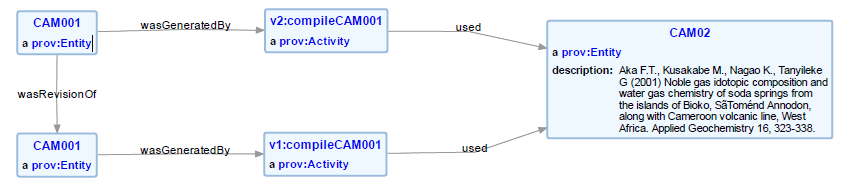
\includegraphics[scale=0.70]{figures/CAM001v1v2.png}
	\caption{Provenance graph for the entry CAM001 entry of the Noble Gas Database.  Other than the labels, the structure of each of the data objects is very much the same.}
	\label{CAM001ProvGraph}
\end{figure}

\section{FORM A MAPPING}

The next step involves formulating a method to determine whether a relationship constitutes an add, invalidate, or modify mapping.
An attribute needs to be identified, which can used as a unique identifier for a piece of datum within the dataset.
In tabular data, this would correspond to the row and column of the datum.
However, new entries into a table rarely takes the form of an individual cell.
Entire rows or columns are usually added as a group.
As a result, when adding or invalidating data
This step largely comes fairly easily to data producers since they have a more comprehensive understanding of the actions taken to create the alternate version.
The key comes down to using the proper attribute identifier.
In a tabular context, this often means using the row or column number, but rows and columns are often rearranged.
Adding or removing a column would 

In the case of the copper minerals dataset, each mineral had a unique name which was used to determine if an entry was removed or added to the dataset.
All names from one version was placed into a set, and all the names of the next version were placed into another set.

So basically, what we do is we figure out what attributes will identify the entries in the data.
Then we compare these sets of attributes to determine if they only exist in one version or both.
The model then tells us how to link together the objects.

For copper

\section{GENERATE VERSIONING GRAPH}

An encoding can now be generated after a method of mapping has been determined.
In current practice, the method of publishing version information comes in the form of a change log.
In this application, the data is published as a versioning graph, leveraging the structure of the concept model.
This allows the data to be stored into a triple store and then retrieved through queries.
In addition, change log and linked data technologies can be combined together into a hybrid artifact using different encoding schemes that embed linked data graphs into documents.
Execution of these hybrid logs had mixed results as very large graphs with many changes became very difficult to load.
As optimization methods are outside the scope of this application, efficiently merging versioning graphs into change logs is not pursued further.
However, in change logs, changes are presented in sections by type.
As a result, when generating the triples, the changes are collected and organized first, then output.

A selection of triples have been extracted from the larger Noble Gas versioning graph in Figure \ref{NobleGraph1}, demonstrating how entries appear.
The graph reads, EGY001 was added, ANC001 no longer appears, and column 11 of CAM001 underwent a modification.
In the case of Figure \ref{NobleGraph1} and \ref{CopperGraphVerGraph}, the graph was extracted from linked data embedded into a change log.
As a result of limitations in the encoding, a unique attribute combining the column number and the row identifier was used to identify the column attribute.
The decision to combine them was to produce an easier graph to run a flow computation on.
An alternative construction would be to use just the column identifier and share it with other entries.
This results in the graph more similar to Figure \ref{NobleGraph2} where column 11 links to multiple changes.

\begin{figure}
	\centering
	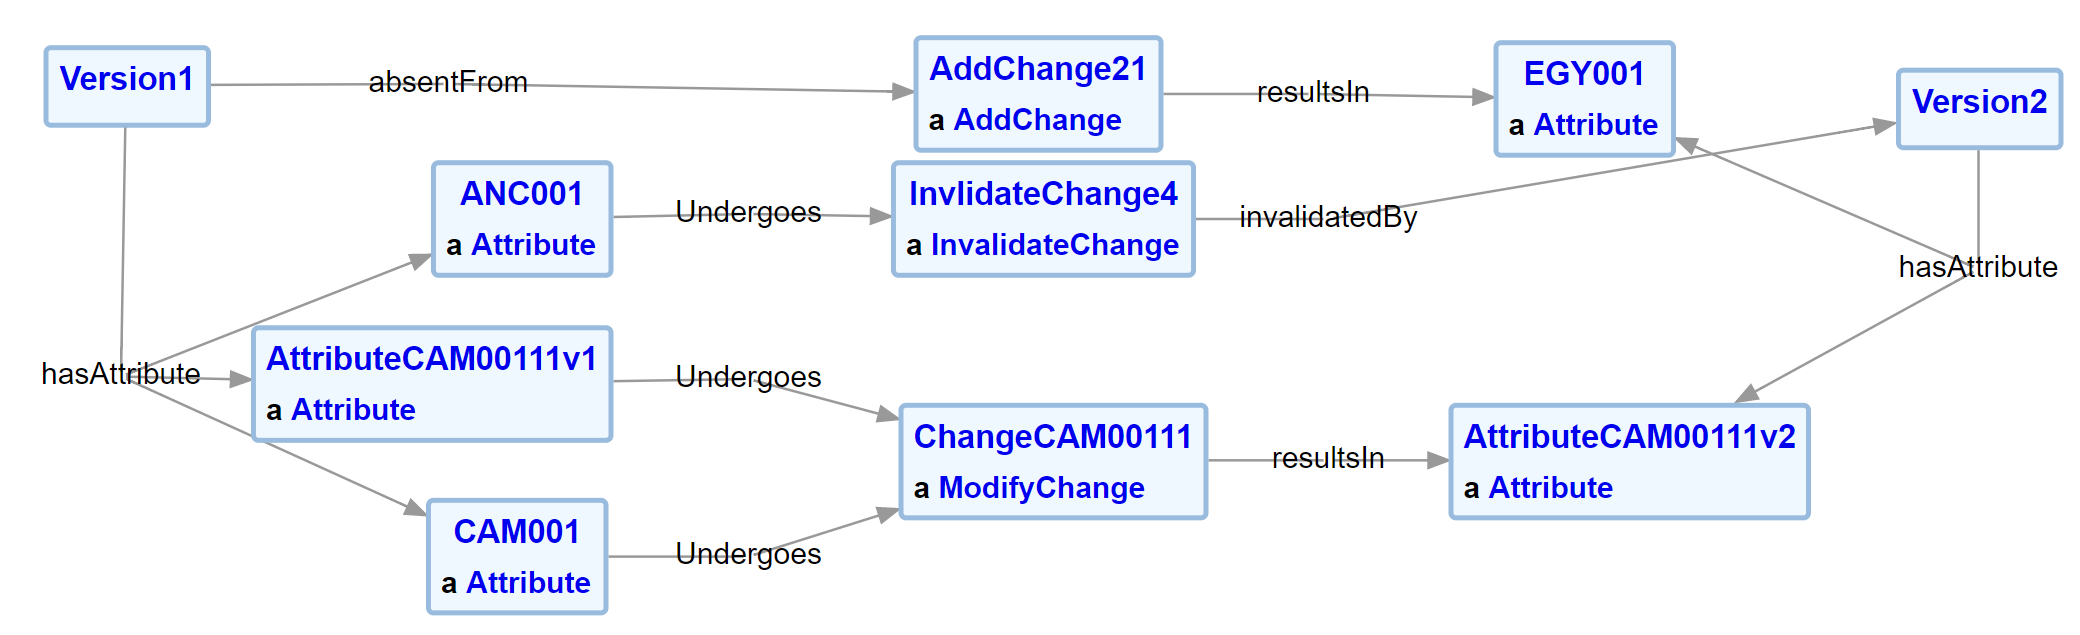
\includegraphics[scale=0.30]{figures/NobleVersion.png}
	\caption{Some initial entries from versions 1 and 2 of the Noble Gas dataset}
	\label{NobleGraph1}
\end{figure}

\begin{figure}
	\centering
	\begin{adjustbox}{addcode={\begin{minipage}{\width}}{
					\caption{Versioning Graph representing the linked data graph with selected entries of additions, invalidations, and modifications. 
			}\end{minipage}},rotate=90,center}
		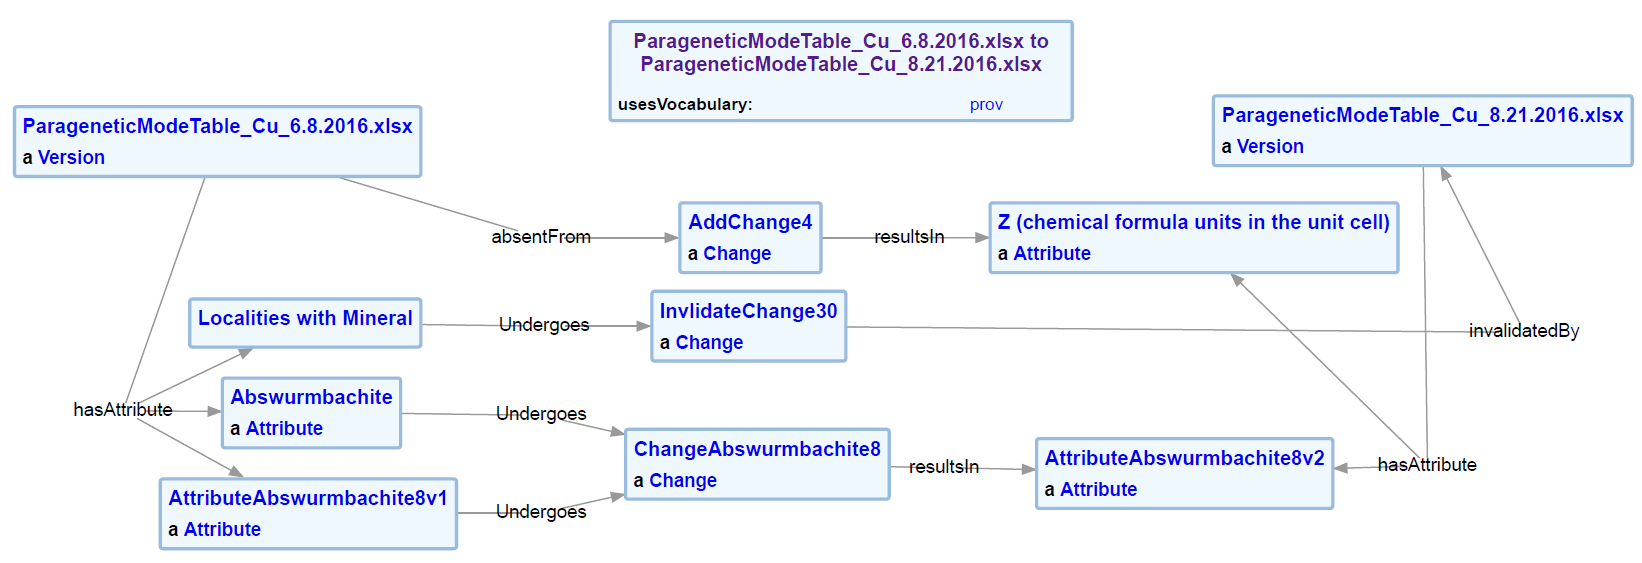
\includegraphics[scale=0.5]{figures/VersioningGraph2.png}%
	\end{adjustbox}
	\label{CopperGraphVerGraph}
\end{figure}

\section{MULTIPLE LINKED VERSIONS}

Versions do not always appear in pairs.
While the figures in this document so far have depicted a comparison between only two versions, versioning often involves more than two objects, either in sequence or parallel.
Using the construction outlined in the previous three sections, many changes can be compiled together into a graph in a changelog.
After all additions, invalidations, and modifications have been compiled into a single graph, a complete mapping from version one to version two may be developed.
The orientation of the relationships in the graph allows a flow to be created from attributes in version one to corresponding attributes in version two.
Taking version two and performing the same graph construction to a version three results in not only a flow from version two to version three, but also from version one to version three.
As a result, the flow can be used to construct a mapping from version one to version three or any future version.

\begin{figure}
	\centering
	\begin{adjustbox}{addcode={\begin{minipage}{\width}}{
					\caption{Versioning Graph representing the linked data graph with selected entries of additions, invalidations, and modifications after the publication of the third version. 
			}\end{minipage}},rotate=90,center}
		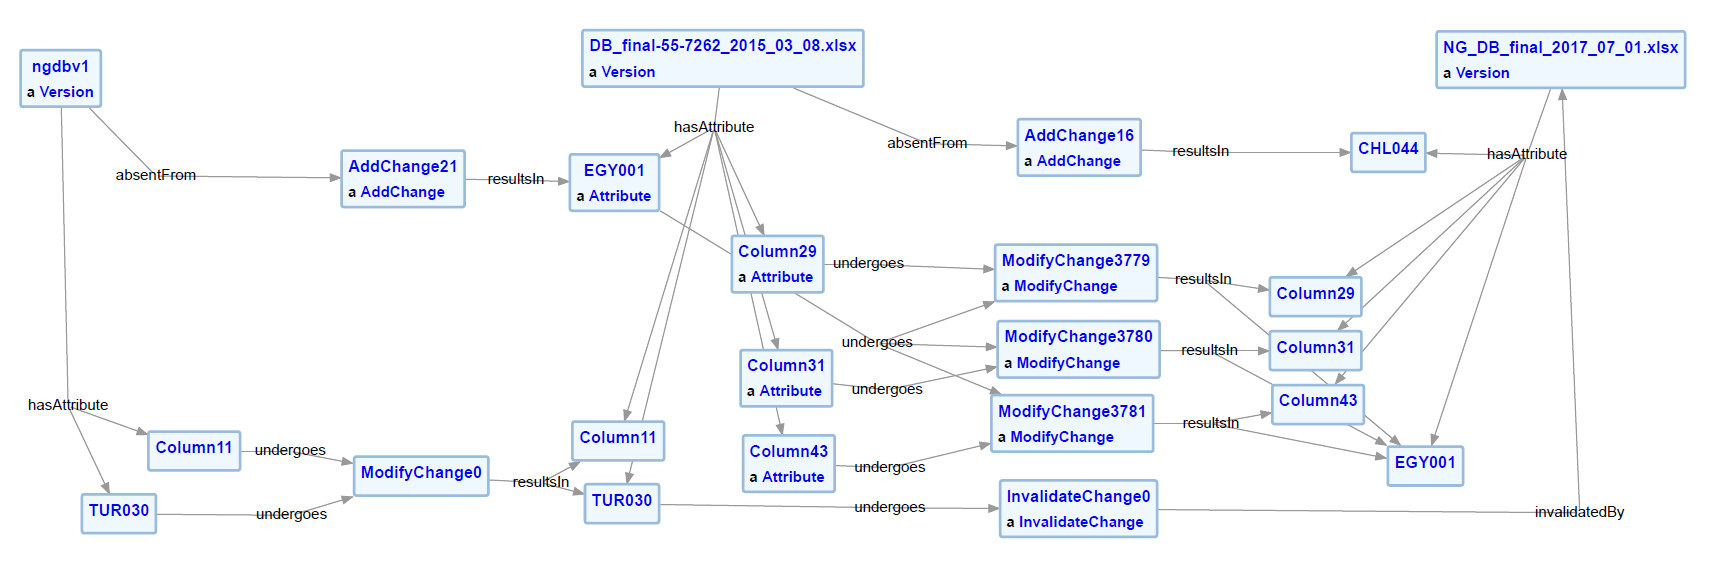
\includegraphics[scale=0.5]{figures/NobleVersion2.png}%
	\end{adjustbox}
	\label{NobleGraph2}
\end{figure}